\chapter{Background}

\newpage

% The Belvedere Glacier (Randolph Glacier Inventory code RGI60--11.02858) is an alpine
% glacier in Valle Anzasca (Italy), on the east side of the Monte Rosa Massif (N
% \ang{45;58} E \ang{7;55}) (\figref{fig:studyarea}). 
% The lower part of the Belvedere Glacier is a temperate debris-covered glacier, that covers an area of
% \SI{\sim1.8}{\kilo\meter\squared} and extends from an altitude of \SI{\sim2250}{\masl} to \SI{\sim1800}{\masl}.
% This region is characterized by a gentle slope, and it is fed by ice falls and snow
% avalanches coming from the Monte Rosa East Face \citep{Haeberli2002}. In its low-relief
% sector, the Belvedere Glacier splits into two lobes, reaching \SI{\sim1800}{\masl}.
% The northern lobe, in particular, ends with a prominent ice cliff, from which the River
% Anza springs.

% Similarly to Miage glacier (Monte Bianco, Valle d’Aosta), the Belvedere Glacier is almost completely covered by rocks and boulders with dimensions ranging from few decimetres to some meters, which makes it a \textit{black glaciers}.
% Due to the global warming trend, the~number of black glaciers along the Italian Alps is rising~\citep{Diolaiuti2003}. 
% Up to the beginning of the century, the~debris cover helped to compensate the effect of the increased temperature, establishing a negative feedback in the temperature-ablation relationship~\citep{Roethlisberger1985,Diolaiuti2003}.
% However, in~recent years, the~debris cover protection has not been sufficient to limit the glacier~retreat.


% \begin{figure}
%     \centering
%     \subcaptionbox{\label{fig:studyarea:map}}{
%         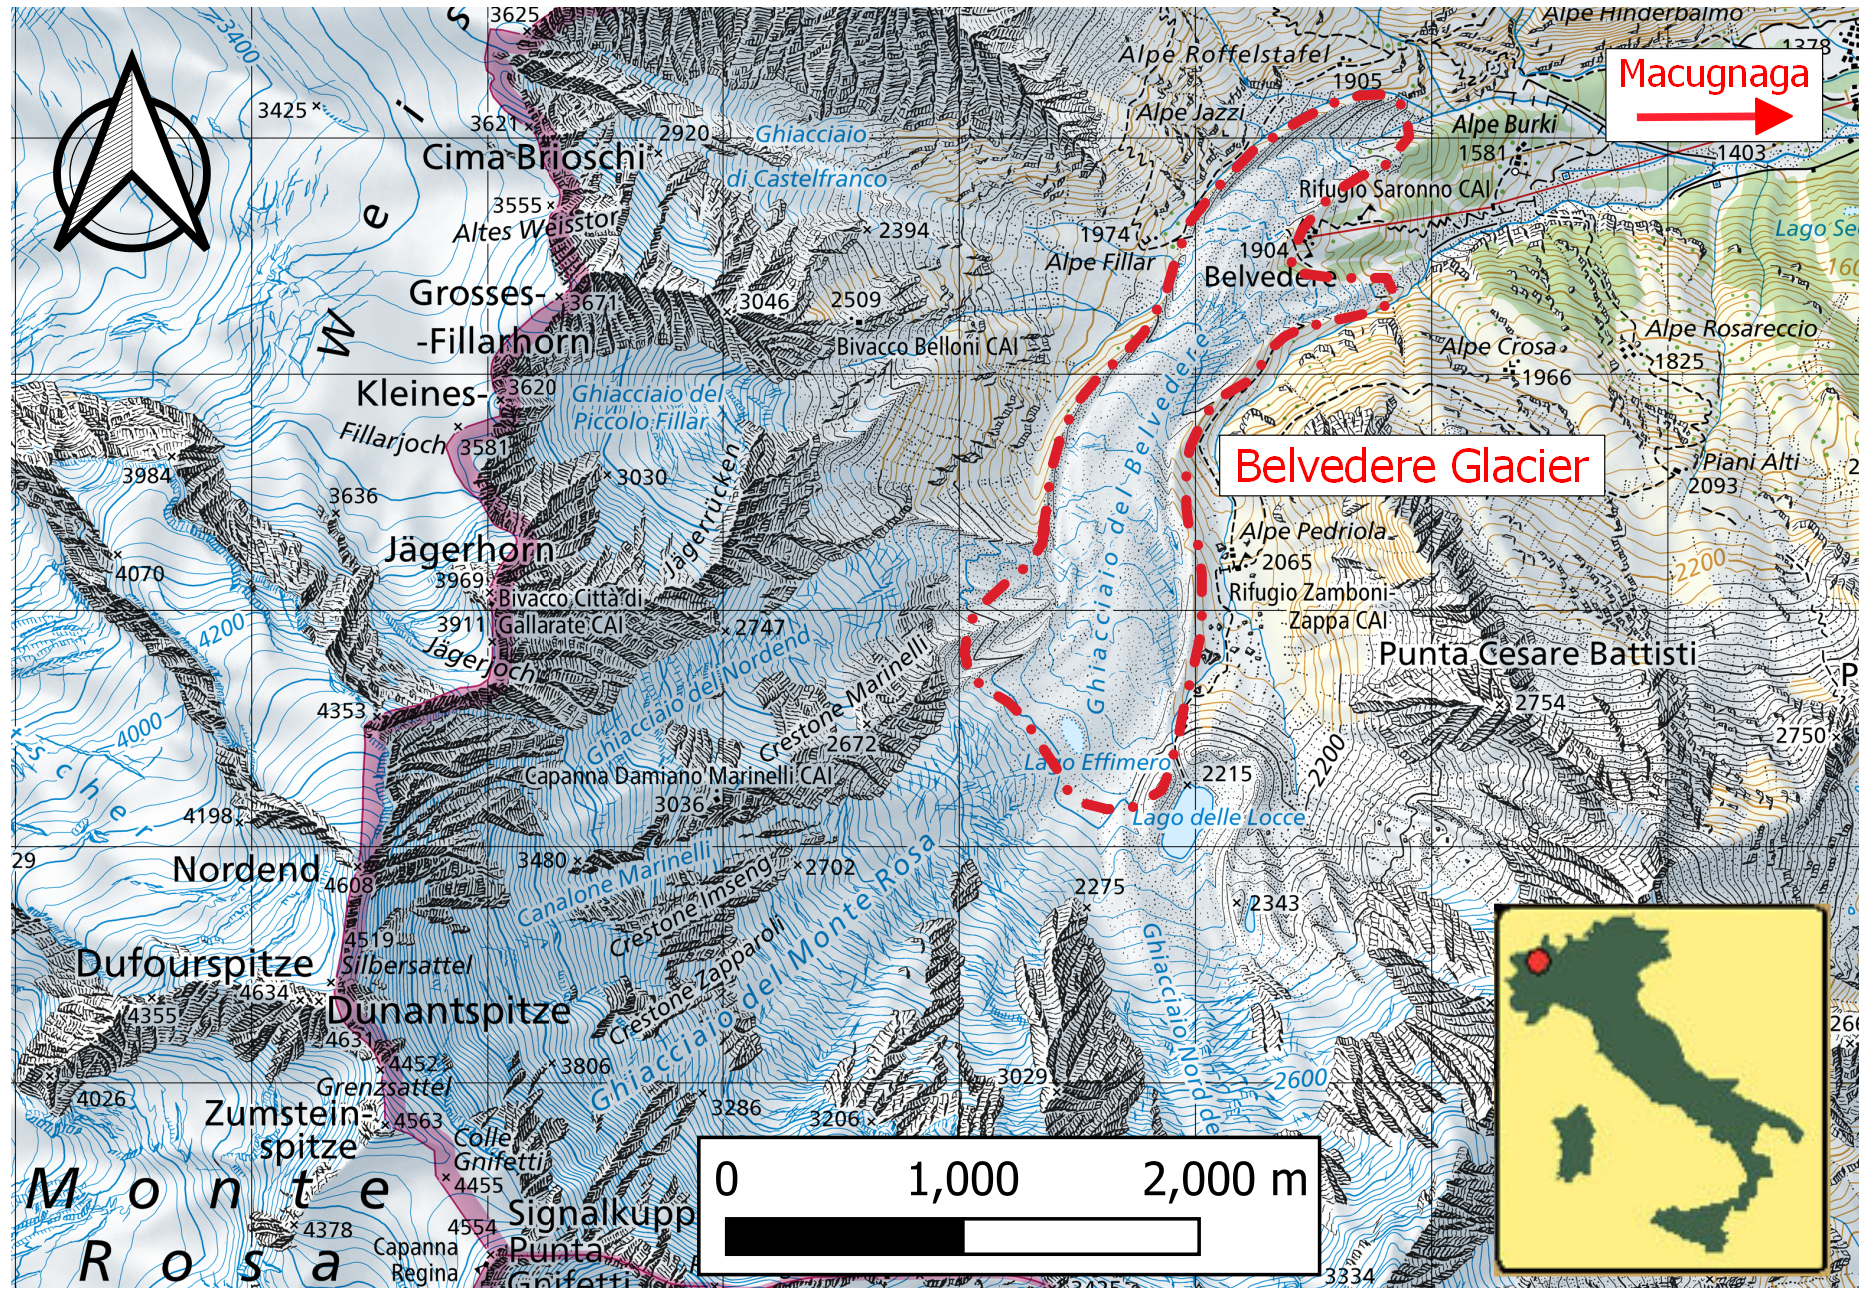
\includegraphics[width=0.48\textwidth]{figures/1_introduction/belvedere_location.png}
%     }
%     \subcaptionbox{\label{fig:studyarea:pic}}{
%         \includegraphics[width=0.48\textwidth]{figures/1_introduction/belvedere_pic.jpg}
%     }
%     \caption{(a) Location of Belvedere Glacier, base map (source: Swisstopo www.geo.admin.ch); (b) Picture of ...}
%     \label{fig:studyarea}
% \end{figure}

% In the past, several hazardous events originated by the Belvedere Glacier, such as floods
% and slope instability, threatened the nearby village of Macugnaga and the Zamboni Zappa Hut,
% at 2070 m a.s.l. \citep{Kaab2004}. 
% At the beginning of the 21st century, the Belvedere Glacier was characterized by a particular 
% surge-type dynamics  \citep{Haeberli2002}. 
% During the late 1990s, the~surface speeds of the whole glacier were ranging between \SIlist{30;45}{\meter\per\year}~\cite{Roethlisberger1985, Kaab2005}.
% During 2000--2001 an accelerated flow in the Monte-Rosa Glacier produced a wave of compression-decompression stresses and strains in the Belvedere Glacier. 
% Surface velocities soared: values up to \SI{200}{\meter\per\year} were observed photogrammetrically during autumn 2001~\cite{Kaab2004}. 
% The ice thickness increased more than~\SI{20}{\meter} and the wave travelled downwards, creating a depression area in the accumulation zone, that was filled by a super-glacial lake, the~Lago Effimero~\cite{Haeberli2002, Mortara2009}.

% The northern lobe of the Belvedere Glacier is concurrently experiencing a fast retreat:
% in the past few years, an average retreat of \SI{\sim20}{\meter\per\year} was documented
% \citep{Ioli2022} and it is actively changing every day, due to ice falls and collapses.


\bibliographystyle{apalike2}
\bibliography{references}
\addcontentsline{toc}{section}{References}